% !TeX root = ./ELNW_PR_Juan2.tex
% !TeX spellcheck = de_DE
%-------------------------------------------%
%--------------- 0_Main.tex ----------------%
%-------------------------------------------%
%----- Hauptteil des LaTeX-Projektes: ------%
%----- Hier werden nacheinander alle -------%
%----- weiteren tex-Dateien eingefügt. -----%
%-------------------------------------------%
%-------------------------------------------%
%----- Achtung: Kapitelüberschriften -------%
%-----          und Verweise werden --------%
%-----          bereits hier erstellt! -----%
%-------------------------------------------%
%-------------------------------------------%
% 
%-----------------------------------------------%
%-------------- 0-0_Packages.tex ---------------%
%-----------------------------------------------%
%----- Enthält alle Packages sowie die ---------%
%----- Voreinstellungen fürs Seitenlayout. -----%
%-----------------------------------------------%
%-----------------------------------------------%
%----- Achtung: Änderungen können weit- --------%
%-----          reichende Folgen haben! --------%
%-----------------------------------------------%
%-----------------------------------------------%
%
\documentclass[
	paper = a4,               % Papierformat
	oneside,                  % einseitig
	fontsize = 12pt,          % Schriftgröße
	headsepline = .5pt,       % untere Kopfzeilenlinie
	numbers = noenddot,       % 1.1.1. --> 1.1.1
	parskip = half,           % halber Absatz
	titlepage = on,           % Titelseite
	captions = tableheading,  % Tabellenüberschriften
	DIV = 12,                 % Satzspiegel (KOMA-Script)
	toc = bibliography,       % Quellenverzeichnis ins Inhaltsverzeichnis aufnehmen
  listof = totoc,
]{scrartcl}
\setcounter{secnumdepth}{4}
\setcounter{tocdepth}{4}

\usepackage[ngerman]{babel}
\addto\captionsngerman{\renewcommand{\refname}{Quellenverzeichnis}}
\usepackage[T1]{fontenc}
\usepackage{lmodern}
\usepackage[utf8]{inputenc}
\usepackage{lipsum} % Erzeugt Blindtext. Kann von euch auskommentiert werden.

% Pakete für Bibtex/Quellenangaben
% Werden bereits hier geladen, weil es sonst zu einer Kollision zwischen zwei Packages kommt.
\usepackage[noadjust]{cite}
\usepackage[hyphens]{url}	% Nutze vorhandene Bindestriche für Zeilenumbrüche in URLs.
\usepackage{etoolbox}
\apptocmd{\sloppy}{\hbadness 10000\relax}{}{}	% Ignoriere Boxen mit zu viel Weißraum im 'sloppy'-Modus.

% Pakete für Formeln
\usepackage{amsfonts}
\usepackage{amsmath}
\usepackage{amssymb}
\usepackage{siunitx}
\sisetup{
  output-decimal-marker = {,},
  inter-unit-product = \ensuremath{{}\cdot{}},
  range-phrase = ...
}
\renewcommand{\theequation}{\arabic{section}.\arabic{subsection}}	% Formeln mit genauer Abschnittangabe beschriften.
\numberwithin{equation}{subsection}  % Die Nummerierung einer Gleichung hinten anhängen.
\newcommand\numberthis{\addtocounter{equation}{1}\tag{\theequation}} % Einzelne Nummerierung innerhalb von 'align*'-Umgebung.

% Pakete für Quellcode und Verzeichnisse
% Werden bereits hier geladen, weil es sonst zu einer Kollision zwischen zwei Packages kommt.
\usepackage{enumerate}
\usepackage[]{listofsymbols}
\usepackage{listings}

\renewcommand{\lstlistlistingname}{Codelistenverzeichnis}
%\usepackage{scrhack}  % Löst Probleme mit veralteten KOMA-Befehlen im 'listings'-Package.
\usepackage{paralist} % Mehr Optionen beim Erstellen von Aufzählungen ('\enumerate').
\usepackage[usenames,dvipsnames]{xcolor}
\lstset{
	basicstyle = \scriptsize\ttfamily,
  keywordstyle = \bfseries\ttfamily\color{NavyBlue},
  stringstyle = \color{violet}\ttfamily,
  commentstyle = \color{green}\ttfamily,
  emph = {square}, 
  emphstyle = \color{blue}\texttt,
  emph = {[2]root,base},
  emphstyle = {[2]\color{yac}\texttt},
  language = c,
  tabsize = 2,
  basicstyle = \footnotesize\ttfamily,
  numbers = left,
  numberfirstline,
  breaklines = true,
  breakatwhitespace = true,
  linewidth = \textwidth,
  xleftmargin = 0.075\textwidth,
  frame = tlrb,
  captionpos = b,
  inputencoding = {utf8},
  extendedchars = false
}

% Pakete für Grafiken
\usepackage{graphicx}
\usepackage{subcaption}
\usepackage{rotating}
\usepackage{float}
\usepackage{picinpar}
\usepackage[section]{placeins}
%\usepackage{hyperref}					    % Wird ganz zum Schluss geladen (s.u.), sonst kommt es zu Warnungen.
\usepackage{microtype}              % Schriftbildverschönerung
\usepackage{textcomp}               % Fügt zusätzliche Symbole im Textmodus ein.
\usepackage[format = hang]{caption} % Einstellungen für Bildunter- bzw. überschriften:
\pdfminorversion = 6

% Pakete für Schaltpläne/Zeichnungen
\usepackage{pgfplots}
\pgfplotsset{compat = 1.13,
             /pgf/number format/.cd,
             use comma,
             1000 sep = {}}
\usepackage{tikz}							    % TIKZ-Paket
\usepackage{circuitikz}					  % Schaltpläne mit TIKZ erstellen.
\usetikzlibrary{matrix,           % Mehr Optionen zum Erstellen und Formatieren von Matrizen.
                shapes,           % Stellt weitere geometrische Formen zur Verfügung.
                arrows.meta,      % Mehr Optionen zum Erstellen und Formatieren von Pfeilen.
                positioning,      % Erweiterte Optionen zum Platzieren von Objekten.
                circuits.ee.IEC,  % Beinhaltet die offiziellen IEC-Schaltzeichen.
                calc}             % Ermöglicht komplexe Berechnungen mit Koordinaten.
\usepackage{marvosym}             % Fügt einige Symbole zur Verwendung in Grafiken hinzu.

% Pakete für Tabellen
\usepackage{array}
\usepackage{tabularx}
\newcolumntype{w}[1]{>{\raggedleft\hspace{0pt}}p{#1}}
\usepackage{bigdelim}         % Ermöglicht bessere Formatierung der Zellen untereinander.
\usepackage{booktabs}         % Ermöglicht besseres Tabellen-Layout.

% Pakete für Style/Formatierung
\usepackage{fancybox}
\usepackage{ulem}
\usepackage{setspace}
\usepackage[a4paper,
            lmargin = {25mm},
            rmargin = {25mm},
            tmargin = {25mm},
            bmargin = {25mm}]{geometry}
\addtolength{\footskip}{-0.8cm}  % Fussbereich 0,8 cm höher, so dass die Seitennummierung höher ist.
\onehalfspacing

% Anhang
\usepackage[title, titletoc]{appendix}

\usepackage{scrlayer-scrpage}				  % KOMA-Paket\usepackage{csvsimple}
\usepackage{tabularx}
\usepackage{siunitx}
\usepackage{physics}
\usepackage{minted}
\usepackage{csvsimple}
\usepackage[pdfpagelabels]{hyperref}	% Muss ganz zum Schluss geladen werden (s.o.).
\usepackage{newtxmath}
\usepackage{scrhack}
%\usepackage[style=authoryear]{biblatex} 
%----------------------------------------------%
%------------ 0-1_Projektdaten.tex ------------%
%----------------------------------------------%
%----- Hier definiert ihr alle benötigten -----%
%----- formalen Angaben zu eurer Arbeit.-------%
%----------------------------------------------%
%----------------------------------------------%
%----- Die Daten werden für Titelblatt, -------%
%----- eidesstattliche Erklärung sowie --------%
%----- Kopf- und Fußzeile verwendet. ----------%
%----------------------------------------------%
%----------------------------------------------%
%
% Angaben zum Thema
\newcommand{\titel}{Ausgleichsvorgang 1. und 2. Ordnung}
\newcommand{\art}{Protokoll}
\newcommand{\termin}{2. Praktikumstermin}
\newcommand{\veranstaltung}{Laborpraktikum}
\newcommand{\modul}{Elektrische Netzwerke}
\newcommand{\semester}{Sommersemester 2021}

% Angaben zum Fachgebiet
\newcommand{\universitaet}{Technische Universität Berlin}
\newcommand{\fakultaet}{Fakultät IV - Elektrotechnik und Informatik}
\newcommand{\institut}{Institut für Energie- und Automatisierungstechnik}
\newcommand{\fachgebiet}{Fachgebiet für Energieversorgungsnetze und Integration Erneuerbarer Energien}

% Angaben zur Person
\newcommand{\autorA}{Juan Nicolas Pardo Martin} % Vorname, Name
\newcommand{\matrikelnrA}{389772}       % Matrikelnummer
% \newcommand{\autorB}{}                % ggf. weitere Autoren (Hier nicht nötig!)
% \newcommand{\matrikelnrB}{}
% ...

% Angaben zur Abgabe
% \newcommand{\dozent}{}                                        % Dozent (Hier nicht nötig!)
\newcommand{\betreuer}{Jeanne Steiner}                   % Laborbetreuer
\newcommand{\labortermin}{Samstag, 30. Mai 2021, 16-18 Uhr} % Labortermin
\newcommand{\abgabedatum}{Montag, den 30. Mai 2021}        % Abgabedatum (lang)
\newcommand{\abgabedatumKurz}{17. Mai 2021}                 % Abgabedatum (kurz)
\newcommand{\ort}{Berlin}                                       % Abgabeort
%-----------------------------------------------------%
%------------------ 0-2_Layout.tex -------------------%
%-----------------------------------------------------%
%----- Hier werden Kopf- und Fußzeile definiert. -----%
%----- Außerdem können Befehle erstellt werden, ------%
%----- die euch später im Hauptteil das Leben --------%
%----- deutlich einfacher machen können. -------------%
%-----------------------------------------------------%
%-----------------------------------------------------%
%
% Kopf- und Fußzeile
\pagestyle{scrheadings}							% Seitenstil
\setkomafont{pagehead}{\normalfont}
\clearscrheadfoot										% Lösche alle Voreinstellungen.
\automark{section}									% Setze Automark auf aktuellen Abschnitt.
\ihead{\titel}                      % Schreibe Thema in die Kopfzeile (innen).
% \chead{\headmark}								  % Schreibe Abschnittsüberschrift in die Kopfzeile (Mitte).
\ohead{\autorA}					            % Schreibe Namen in die Kopfzeile (außen).
\cfoot{\pagemark}										% Erstelle (zentrale) Seitennummern.

% Hier können z.B. bequem neue Einheiten für das 'siunitx'-Package definiert werden.
% Passt auf, dass ihr dabei keine vorhandenen Einheiten überschreibt!
%
% \DeclareSIUnit{\voltampere}{VA}
% \DeclareSIUnit{\ah}{Ah}
% \DeclareSIUnit{\wh}{Wh}

% Mit Befehlen können z.B. Abkürzungen für langwierige Formeln o.Ä. erstellt werden.
% Passt auch hier auf, dass ihr nichts überschreibt!
%
% \newcommand{\uin}{\ensuremath{\underline{U}_\mathrm{e}}}
% \newcommand{\uout}{\ensuremath{\underline{U}_\mathrm{a}}}

% Mit dem 'tikz'-Package könnt ihr u.a. (Ersatz-)Schaltbilder zeichnen. Damit die einigermaßen gut aussehen, kann man z.B. Vorlagen für Schaltsymbole, Spannungs- und Strompfeile definieren. Bitte lasst die vorgegebenen Einstellungen stehen, weil spätere Protokollvorgaben darauf aufbauen werden!
%
%--- Ordentliche Proportionen für passive Grundelemente ---%
%
\tikzset
{
  resistor IEC graphic/.style =
  {
    circuit symbol open,
    circuit symbol size = width 2.5 height 1,
    shape = rectangle ee,
    transform shape
  },
  var resistor IEC graphic/.style =
  {
    circuit symbol lines,
    circuit symbol size = width 3.6 height 0.8,
    shape = var resistor IEC,
    transform shape,
    outer sep = 0pt,
    cap = round
  },
  inductor IEC graphic/.style =
  {
    circuit symbol lines,
    circuit symbol size = width 3 height .5,
    transform shape,
    shape = inductor IEC,
    outer sep = 0pt,
    cap = round
  },
  var inductor IEC graphic/.style =
  {
    circuit symbol filled,
    circuit symbol size = width 2.5 height 1
    transform shape,
    shape = rectangle ee
  },
  capacitor IEC graphic/.style =
  {
    circuit symbol lines,
    circuit symbol size = width .5 height 1.5,
    transform shape,
    shape = capacitor IEC
  }
}
%
% --- Messgeräte ---%
%
\tikzset
{
  circuit declare symbol = amperemeter,
  set amperemeter graphic =
  {
    draw,
    generic circle IEC,
    minimum size = 10mm,
    info = center:A
  },
  circuit declare symbol = voltmeter,
  set voltmeter graphic =
  {
    draw,
    generic circle IEC,
    minimum size=10mm,
    info = center:V
  }
}
%
%--- Pfeile ---%
%
\tikzset{
  DickerPfeil/.style = {ultra thick, shorten >= #1, shorten <= #1, -{Straight Barb[angle' = 60, scale = 1.5]}},
	UPfeil/.style = {blue, DickerPfeil = #1, font = {\sffamily\itshape}},
  IPfeil/.style = {red, DickerPfeil = #1, font = {\ttfamily\itshape}}
}
%
\begin{document}
%-------------------------------------%
%-------- 0-3_Titelblatt.tex ---------%
%-------------------------------------%
%----- Hier wird das Titelblatt ------%
%----- eures Dokuments erstellt. -----%
%-------------------------------------%
%-------------------------------------%
%
\thispagestyle{plain}
%
\begin{titlepage}
  \begin{center}
    
\includegraphics[width = 3.3cm]{setup/Logo_TUB_rot}\hspace{6cm}
    
\includegraphics[width = 2.7cm]{setup/Logo_SENSE}\hspace{1cm}\\[0.5cm]
    \universitaet\\
    \fakultaet\\
    \institut\\
    \fachgebiet
  \end{center}
  %
  \vspace{0.5cm}
  %
  \begin{center}
    \LARGE{\textsc{\titel}}\\[3ex]
    \Large{\textbf{\art}}\\[1ex]
    \large{zum \termin}\\[3ex]
    \Large{\textbf{im \veranstaltung}}\\[3ex]
    \large{des Moduls}\\[1ex]
    \Large{\textbf{\modul}}\\[1ex]
    \large{im \semester}\\[6ex]
    \normalsize
    \begin{tabular}{w{5.4cm}p{8cm}}\\
      Autor:	        & \quad \autorA \ (\matrikelnrA)\\[1.2ex]
      % ggf. Autoren: & \quad \autorA \ (\matrikelnrA)\\[1.2ex]
      %               & \quad \autorB \ (\matrikelnrB)\\[1.2ex]
      %               ...
      % ggf. Dozent: & \quad \dozent\\[1.2ex]
      Betreuer:       & \quad \betreuer\\[1.2ex]
      Labortermin:    & \quad \labortermin\\[1.2ex]
      Eingereicht am: & \quad \abgabedatum\\[3ex]
    \end{tabular}
  \end{center}
\end{titlepage}
\pagestyle{empty}
%-------------------------------------------------------------%
%------------- 0-4_EidesstattlicheErklaerung.tex -------------%
%-------------------------------------------------------------%
%----- Hier wird die eidesstattliche Erklärung erstellt. -----%
%-------------------------------------------------------------%
%-------------------------------------------------------------%
%----- Achtung: Eure Protokollabgabe ist nur mit eurer -------%
%-----          Unterschrift inkl. Datum und Ortsangabe ------%
%-----          gültig - und damit bewertbar! ----------------%
%-------------------------------------------------------------%
%-------------------------------------------------------------%
%
\section*{Eidesstattliche Erklärung}
Hiermit erkläre ich an Eides statt, dass ich die mit meinem Namen gekennzeichneten Teile für das vorliegende \textit{\art}
\bigskip
%
\begin{center}
  \large{\textsc{\titel}}
\end{center}
%
\bigskip
zum \textit{\termin} im \textit{\veranstaltung} des Moduls \textit{\modul} selbstständig und eigenhändig sowie ohne unerlaubte fremde Hilfe und ausschließlich unter Verwendung der aufgeführten Quellen und Hilfsmittel angefertigt habe.

\bigskip

\ort , \abgabedatumKurz

\bigskip
\bigskip

\rule[-0.2cm]{8cm}{0.5pt}

\textsc{\autorA\ (\matrikelnrA)}
%
% \bigskip
%
% \rule[-0.2cm]{8cm}{0.5pt}
%
% \textsc{\autorB\ (\matrikelnrB)}
%
% \bigskip
%
% ...

%
%
%
\newpage
%
\tableofcontents
%
\newpage
\pagestyle{headings}
%
\section{Einleitung}
\label{sec:Einleitung}
%----------------------------%
%----- 1_Einleitung.tex -----%
%----------------------------%
%----------------------------%
%
%\lipsum[2-4]
\par Resonanz ist eine Phänomen, wo bei einer bestimmte Frequenz die Dämpfung (einer Kraft) relativ klein oder 0 ist, Die Energie des systems kann \enquote{unendlich} groß werden. Resonanz ist wenn die Anregung periodisch ist und ihre Frequenz ähnlich wie die Eigenfrequenz des System ist, bekommt man Resonanz.
\par Zum Beispiel wenn man eine Schaukel oder eine Brücke schwingt, oder eine LC Schaltung wenn eine Elektromagnetische Welle induziert eine Spannung mit der Gleiche Frequenz wie die Eigenfrequenz. 

%
% Bitte denkt daran, eure Autorenschaft namentlich zu kennzeichnen! Das gilt für jeden (Unter-)Abschnitt, den ihr bearbeitet habt.
%
\begin{flushright}
  \textit{\autorA}
\end{flushright}
%
%
%

\clearpage
%
\section{Versuchsdurchführung}
\label{sec:Durchführung}
%--------------------------------------%
%----- 3_Versuchsdurchführung.tex -----%
%--------------------------------------%
%--------------------------------------%
%
\subsection{Messung}
\label{subsec:3_Messung}
%
%------------------------------%
%----- Beginn eures Teils -----%
%------------------------------%
%
\begin{itemize}
    \item einen Widerstand ($1\si{\kilo\ohm}$), 
    \item Doppelbanenstecker
    \item Zweitor,
    \item BNC-Bananenstecker
    \item ein BNC-BNC-Kabel 
    \item ein Oszilloskop, 
    \item einen Funktionsgenerator, 
    \item ein Steckbrett,
    \item Steckbrettkabeln
\end{itemize}

Zuerst erhalten wir alle Materialien, dann stellen wir sicher, dass wir notieren, welche Pole wir als Tore betrachten. Nachdem wir die Tore ausgewählt haben, zählen wir unsere Pole wie folgt auf: 1,1', 2,2'

Um die Spannung zwischen 2 beliebigen Polen zu messen, schließen wir beim Messen einen Shunt-Widerstand in Reihe an. Dadurch wird sichergestellt, dass wir später herausfinden können, wie hoch der Strom ist.

Um die Spitze-Spitze-Werte anzuzeigen, drückt man  \enquote{$V_{pp}$}. Für den Zeitunterschied: \enquote{Timedelay}

Der Versuch besteht aus zwei Teilen.
\par Im ersten Teil wird der Funktionsgenerator über einen  ($1\si{\kilo\ohm}$) Shunt-Widerstand mit dem ersten Gate der Blackbox verbunden. Mit dieser Konstruktion können wir die Impedanzmatrixeinträge $Z_{11}$ und $Z_{21}$ bestimmen. Mit dem Oszilloskop wird die Potentialdifferenz des Funktionsgenerators ($U_{Epp}$) und der Pole des ersten Tores ($U_{1pp})$ gemessen. Mit der Differenz dieser beiden Spannungen können wir den Shunt-Widerstand bestimmen. Mit der Zeitdifferenz $\Delta t_{11}$ zwischen $U_{Epp}$ und $U_{1pp}$ kann die Phase des Stromes berechnet werden, danach wird das zweite Tor angeschlossen um $U_{2pp}$ und $\Delta t_{21}$ zu bestimmen.

\par Der zweite Teil ist analog zum ersten Teil, wir wiederholen alle Schritte, die wir für den ersten Teil für das zweite Tor gemacht haben, aber wir ändern $U_{1pp}$ mit $U_{2pp}$ und bestimmen so $Z_{12}$, $Z_{22}$ und $\Delta t_{12}$.
%
%
%
\begin{flushright}
  \textit{\autorA}
\end{flushright}
%
%------------------------------%
%------ Ende eures Teils ------%
%------------------------------%
%
%
%
\subsection{Simulation}
\label{subsec:3_Simulation}
%
%------------------------------%
%----- Beginn eures Teils -----%
%------------------------------%
%
\begin{figure}[H]
    \centering
    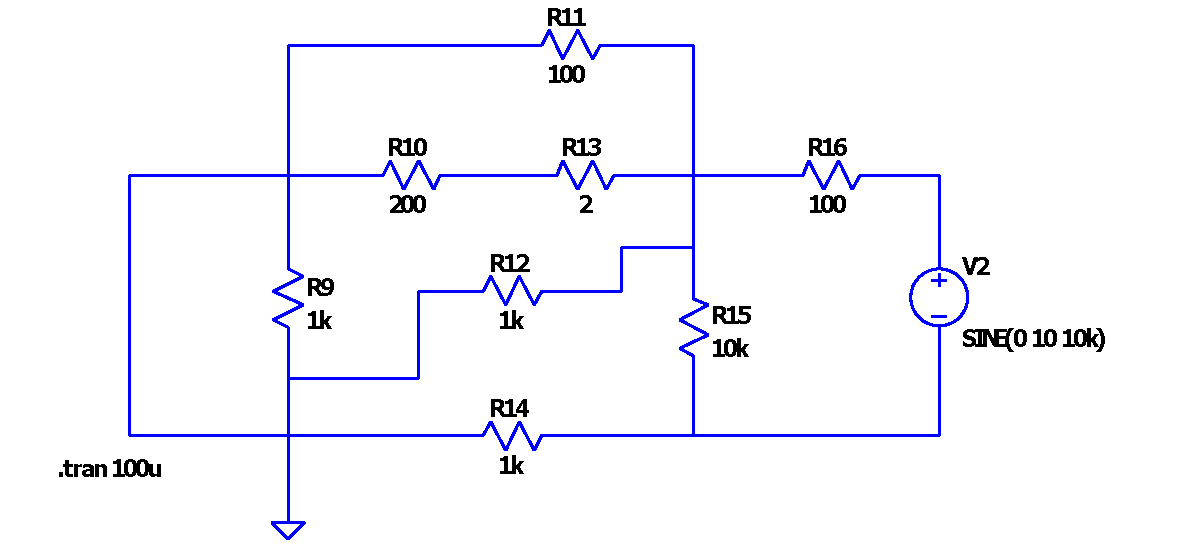
\includepdf[pages={1},scale=.8,pagecommand={}]{src/Schaltung4-1.pdf}
    \caption{LTSpice Simulation 1ste Tor}
    \label{fig:LTSpice1}
\end{figure}
\newpage
\begin{figure}[H]
    \centering
    \includepdf[pages={2},scale=.8,pagecommand={}]{src/Schaltung4-1.pdf}
    \caption{LTSpice Simulation 2te Tor}
    \label{fig:LTspice2}
\end{figure}
\newpage
Für die Simulation haben wir zwei Schaltungen gebaut, eine für das erste Tor und eine für das zweite Tor, Wir führen eine "Transient" simulation durch, von nur $100\si{\micro\second}$. Um die Spannungen bzw Strome (beispielweise $U_1,I_1$) können wir in LTSpice Maschenregel bzw Knotenregel benutzen, exportieren wir diese Werte, mit denen wir die folgenden Diagramme plotten können
\begin{figure}[H]
    \centering
    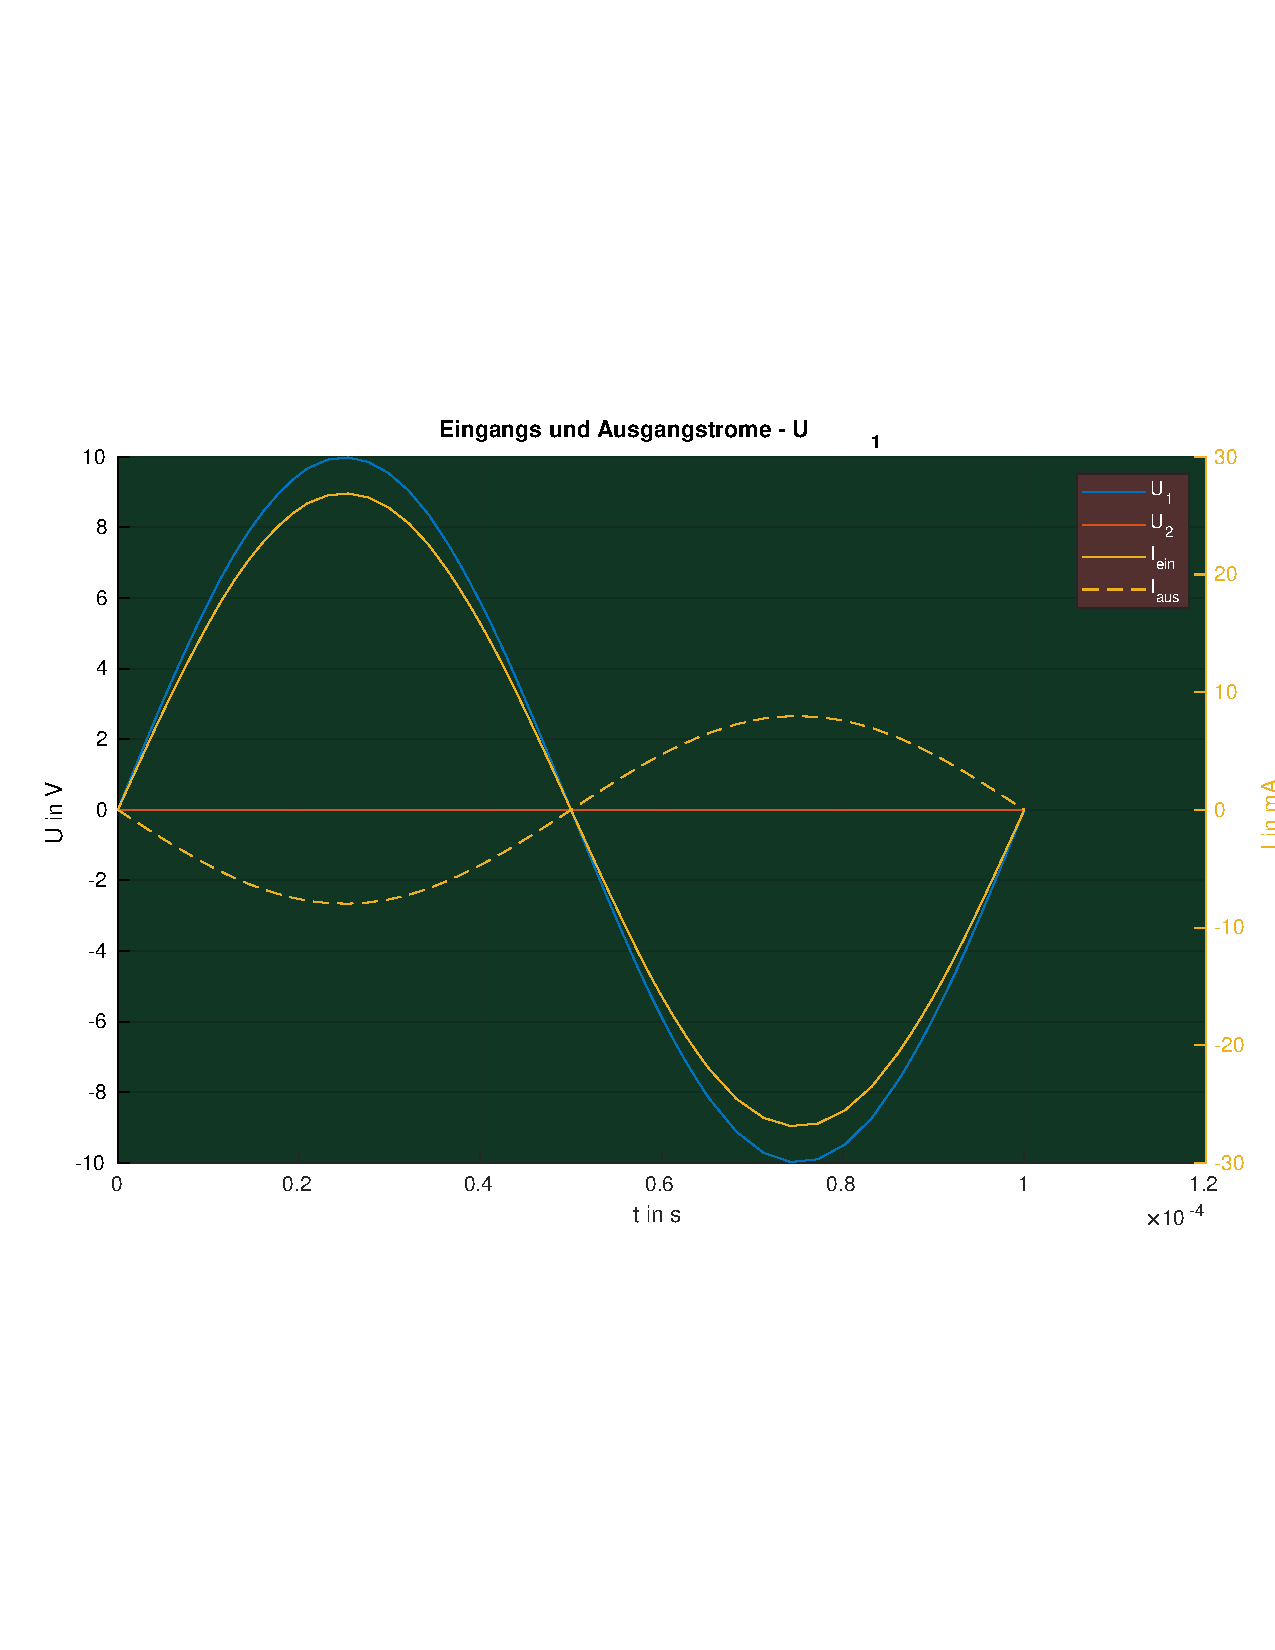
\includegraphics[clip,trim=20pt 200pt 0 200pt,scale=.8]{src/einausgangU_1.pdf}
    \caption{Eingangspannung $U_1$}
    \label{fig:Simulationplot}
\end{figure}
\begin{figure}[H]
    \centering
    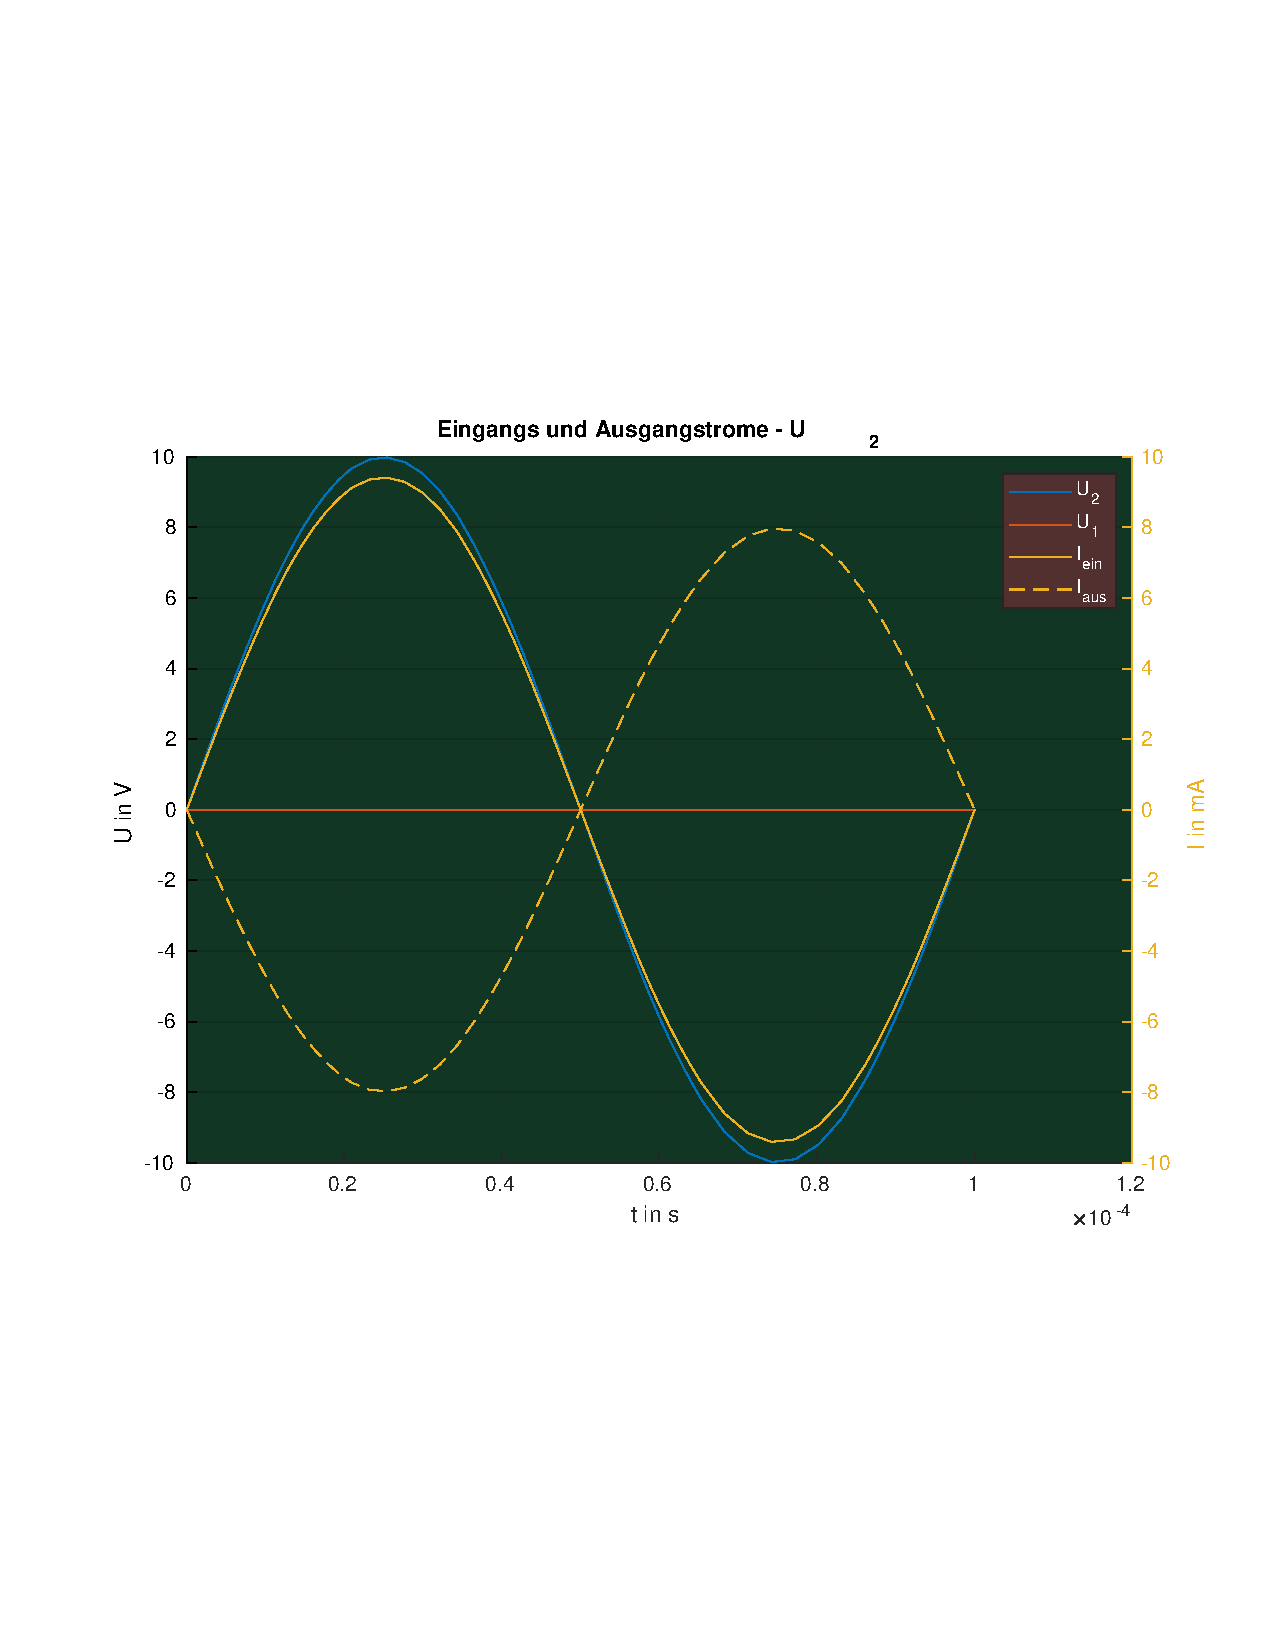
\includegraphics[clip,trim=50pt 200pt 20pt 200pt,scale=.8]{src/einausgangU_2.pdf}
    \caption{Eingangspannung $U_2$}
    \label{fig:Simulationplot2}
\end{figure}
%
\begin{flushright}
  \textit{\autorA}
\end{flushright}
%
%------------------------------%
%------ Ende eures Teils ------%
%------------------------------%
%
%
%
\clearpage
%
\section{Versuchsergebnisse}
\label{sec:Ergebnisse}
%------------------------------------%
%----- 4_Versuchsergebnisse.tex -----%
%------------------------------------%
%------------------------------------%
%
\subsection{Messdaten}
\label{subsec:4_Daten}
%
Zur Bestimmung der Spannung über dem Widerstand $R$ zum Zeitpunkt $t_\mathrm{k}$ wurde die Maschengleichung der Schaltung aufgestellt; der Strom ergab sich aus dem Ohmschen Gesetz am Widerstand $R$:
%
\begin{align*}
   &u_\mathrm{R}(t_\mathrm{k}) = u_\mathrm{E}(t_\mathrm{k}) - u_\mathrm{C}(t_\mathrm{k})
  \numberthis
  \label{eq:4_ur}
  \\
  &i(t_\mathrm{k}) = \frac{u_\mathrm{R}(t_\mathrm{k})}{R}
  \numberthis
  \label{eq:4_i}
\end{align*}
%
Die Messergebnisse sind in Tab. \ref{tab:4_Messdaten} dargestellt\footnote{Alle Werte aufgenommen bzw. berechnet von \autorA}.
%
\begin{table}[H]
  \small
  \centering
	\caption{Messergebnisse}
	\label{tab:4_Messdaten}
	\begin{tabular}{rrrrrr}
	  \toprule
		%
	  \multicolumn{2}{c}{Einstellwerte} &
		\multicolumn{2}{c}{Messwerte} &
		\multicolumn{2}{c}{Berechnete Werte} \\
		\cmidrule(lr{1mm}){1-2}\cmidrule(lr{1mm}){3-4}\cmidrule(lr{1mm}){5-6}
		%
		$t_\mathrm{mess}$ in \si{\micro\second} &
		$t_\mathrm{tat}$ in \si{\micro\second} &
		$u_\mathrm{E}$ in \si{\volt} &
    $u_\mathrm{C}$ in \si{\volt} &
    $u_\mathrm{R}$ in \si{\volt} &
		$i$ in \si{\milli\ampere}\\
		\midrule
		%
		%------------------------------%
    %----- Beginn eures Teils -----%
    %------------------------------%
    %
    \input{src/3_Messwerte.txt}
    % \csvreader[late after line=\\,separator=semicolon]{src/messwertelab1p.csv}{}%
    %{\csvlinetotablerow}%

    %
    \midrule
    %
    % Daten des Ausschaltvorgangs
    %

    %
    %------------------------------%
    %------ Ende eures Teils ------%
    %------------------------------%
    %
		\bottomrule
	\end{tabular}
\end{table}
%
%
%
\newpage
\subsection{Ergebnisplots}
\label{subsec:4_Plots}
%
%------------------------------%
%----- Beginn eures Teils -----%
%------------------------------%
%

%
%
%
%\begin{flushright}
  %\textit{\autorA}
%\end{flushright}
%
%------------------------------%
%------ Ende eures Teils ------%
%------------------------------%
%
%
%
\clearpage
%
\section{Versuchsauswertung}
\label{sec:Auswertung}
%------------------------------------%
%----- 5_Versuchsauswertung.tex -----%
%------------------------------------%
%------------------------------------%
%
%------------------------------%
%----- Beginn eures Teils -----%
%------------------------------%
%
%
%
In diese Simulation haben wir eine Eingangwechselspannung von mit Frequenz, bei den ersten Teil sehen wir, dass wir keine Phasenverschiebung überhaupt, weil wir keine einzige Spule oder Kondensator haben, nur reine Widerstände, wenn wir nur Reelle Impedanzen haben, erwarten wir keine Imaginärteile.

Wir können sehen, bei der Betrachtung der Impedanzmatriz, dass die Komponenten $Z_{12}$ und $Z_{21}$ nach der Theorie gleich seien sollen, aber das ist hier nicht den fall, das kann an der Messabweichung unsere Zeitmessung liegen. Interessanterweise ist die Eingangspannung ein bisschen kleiner im Zweiten teil des Versuchs im vergleich zu ersten Teil, dies könnte darauf zurückgeführt werden, dass bei der Zweite versuch mehr Strom fließt, das könnte verursachen, dass die Signalgenerator die Spannung begrenzt. 

%
\begin{flushright}
  \textit{\autorA}
\end{flushright}
%
%------------------------------%
%------ Ende eures Teils ------%
%------------------------------%
%
%
%
\clearpage
%
\section{Zusammenfassung}
\label{sec:Zusammenfassung}
%---------------------------------%
%----- 6_Zusammenfassung.tex -----%
%---------------------------------%
%---------------------------------%
%
%------------------------------%
%----- Beginn eures Teils -----%
%------------------------------%
%
Das Wichtigste ist zu erkennen, was die Bedeutung der Ordnung einer Schaltung bedeutet und wie sie der Ordnung der DGL entspricht, die wir lösen müssten, um den Zustand der Schaltung zu jedem Zeitpunkt zu beschreiben. Wir lernen auch Ausgleichvorgänge kennen, bei denen die Schaltkreise von einem Zustand in einen anderen übergehen, aber dank Kondensatoren oder Induktivitäten von einem Zustand in den anderen "glatt" übergehen. Wir lernen auch, dass die Theorie immer ein bisschen unpassend sein wird als das, was wir tatsächlich messen werden.



%
%
%
\begin{flushright}
  \textit{\autorA}
\end{flushright}
%
%------------------------------%
%------ Ende eures Teils ------%
%------------------------------%
%
%
%
\clearpage
%

% Tabellenverzeichnis
\listoftables
\newpage
%
% Abbildungsverzeichnis
\listoffigures
\newpage
%
% Codelistenverzeichnis (Bitte bei Nichtverwendung auskommentieren!)
%\lstlistoflistings
%\newpage
%
% Quellenverzeichnis
%---------------------------------------------------------%
%-------------------- 0-5_Quellen.tex --------------------%
%---------------------------------------------------------%
%----- Hier sollt ihr eure Quellen angeben. --------------%
%---------------------------------------------------------%
%---------------------------------------------------------%
%----- Achtung: Direkte und indirekte Zitate müssen ------%
%-----          in jedem Fall gekennzeichnet werden. -----%
%-----          Verstöße werden als Betrugsversuch -------%
%-----          und entsprechend mit 0 PP bewertet! ------%
%-----          Außerdem kann ein Plagiatsvorwurf zu -----%
%-----          weiteren Untersuchungen führen! ----------%
%---------------------------------------------------------%
%---------------------------------------------------------%
%
%\begin{sloppy}
%\begin{small}
%\begin{onehalfspacing}
  %\begin{thebibliography}{--------------------} % Bestimmt den Platz, den Bezeichner erhalten.
  %%
  %% Am besten alphabetisch nach dem Bezeichner ('[Xyz]') sortieren!
  %%
  %%
  %%
%%
%% Vorlagen:
%%
  %%\bibitem[]{src:}
    %%: \glqq \grqq, , \\
    %%\url{}\\
    %%Stand:
  %%
  %% ODER:
  %%
  %%\bibitem[]{src:}
    %%: \glqq \grqq, , \\
    %%\url{}\\
    %%Zugriff: , Uhr
  %\end{thebibliography}
%\end{onehalfspacing}
%\end{small}
%\end{sloppy}

\newpage
%
% Anhang (Bitte bei Nichtverwendung auskommentieren!)
%\appendices
%--------------------------------------------------------%
%-------------------- 0-6_Anhang.tex --------------------%
%--------------------------------------------------------%
%----- Hier könnt ihr weiterführende Informationen, -----%
%----- umfangreiche Codelisten, Messdatensammlungen -----%
%----- oder andere Quellmaterialien einfügen. -----------%
%--------------------------------------------------------%
%--------------------------------------------------------%
%----- Achtung: Fügt bitte ausschließlich Inhalte -------%
%-----          ein, die wirklich relevant für eure -----%
%-----          Ausführungen sind! ----------------------%
%--------------------------------------------------------%
%--------------------------------------------------------%
%
\section{Verwendeter Matlab-Code}
\label{app:Matlab}
%
\begin{minted}[mathescape,
               linenos,
               numbersep=3pt,
               gobble=0,
               frame=lines,
               framesep=2mm,breaklines]{matlab}
t=readLTspice("./labor2.txt","Nyquist")
figure(1)
clf
subplot(2,1,1);
plot(t(:,1)*1e3,t(:,2))
hold on
plot(t(:,1)*1e3,t(:,3))
plot(t(:,1)*1e3,t(:,4))
grid on
xlabel("t in ms")
ylabel("U in V")
title("Spannungen der RC-Parallelschaltung" )
legend('U_E','U_{C_1}',"U_{C_2}")
hold off
subplot(2,1,2);
plot(t(:,1)*1e3,t(:,5)*1e3)
hold on
plot(t(:,1)*1e3,t(:,6)*1e3)
plot(t(:,1)*1e3,t(:,7)*1e3)
xlabel("t in ms")
ylabel("I in mA")
title("Strömungen der RC-Parallelschaltung" )
legend('I_{U_E}','I_{C_1}',"I_{C_2}")
grid on
messwerte=load('ELNW_PR_02_Vorgabe_Messwerte.mat')
messwerte.I_ges=(messwerte.u_E-messwerte.u_C)
R = 1e3;
C = 100e-9;
%für Idealität
t_ideal = [-0.1 0 0 0.5 0.5 1]
uE_ideal = [0 0 10 10 0 0];

% die ideale Aufladevorgang 
t1 = (0:0.01:0.5)*1e-3;                     
U_E1 = 10;

uC_ideal_EIN = U_E1 * (1-exp(-1/(R*C) * t1));

% Entladevorgang
t2 = (0.5:0.01:1) *1e-3;                  
t0 = 0.5e-3;                               
U_E2 = 10;                               

uC_ideal_AUS = U_E2 * exp(-1/(R*C) * (t2-t0));


tC_ideal = [t1 t2]*1e3;                 
uC_ideal = [uC_ideal_EIN uC_ideal_AUS];


uR_ideal_AUS = 0 - uC_ideal_AUS;
uR_ideal_EIN = 10 - uC_ideal_EIN;
uR_ideal = [uR_ideal_EIN uR_ideal_AUS];
i_ideal = uR_ideal;


figure(2)
clf
%plot(messwerte.t_mess,'DisplayName','t_mess');
hold on;
plot(messwerte.t_mess,messwerte.u_C,'bx','DisplayName','u_C');
plot(tC_ideal,uC_ideal,'b-','DisplayName','u_C Ideal');

plot(messwerte.t_mess,messwerte.u_E,'rx','DisplayName','u_E');
plot(t_ideal,uE_ideal,'r-','DisplayName','u_E Ideal');
ylabel("U in V")
yyaxis right
plot(messwerte.t_mess,messwerte.I_ges,'yx','DisplayName','I_{ges} U_R');
plot(tC_ideal,uR_ideal,'y-','DisplayName','I_{ges} U_R Ideal');
ylabel("I in mA")
legend()
%legend("u_C","u_E","I_{ges}, U_R")
xlabel("t in ms")
title("Messwerte für RC-Schaltung")
hold off;
\end{minted}

\section{Verwendeter Python-Code}
\label{app:Python}
%\inputminted{python}{src/reader.py}
%
%
%
% Auch im Anhang sollte die Autorenschaft gekennzeichnet werden. Ihr könnt aber im Falle von Scilab-Code die Autorenschaft im Code selbst kennzeichnen.
%
\begin{flushright}
  \textit{\autorA}
\end{flushright}
%
%
%
%\newpage
%\section{Datenblätter}
%\label{app:Datenblätter}
%
%\lipsum[7-9]
%
%
%
% Auch wenn es sich nur um Abbildungssammlungen handelt, muss die Autorenschaft trotzdem gekennzeichnet werden.
%
%\begin{flushright}
  %\textit{\autorA}
%\end{flushright}
%
%
%
%
\end{document}
%
%------------------------------------------%
%------------------------------------------%
%----- Autor:   Martin Otto           -----%
%------------------------------------------%
%----- FG SENSE, Fak. IV, TU Berlin   -----%
%------------------------------------------%
%----- Version: 1.0.0                 -----%
%----- Datum:   03.05.2018, 11.30 Uhr -----%
%------------------------------------------%
%------------------------------------------%